\begin{figure*}[t]
	\centering
	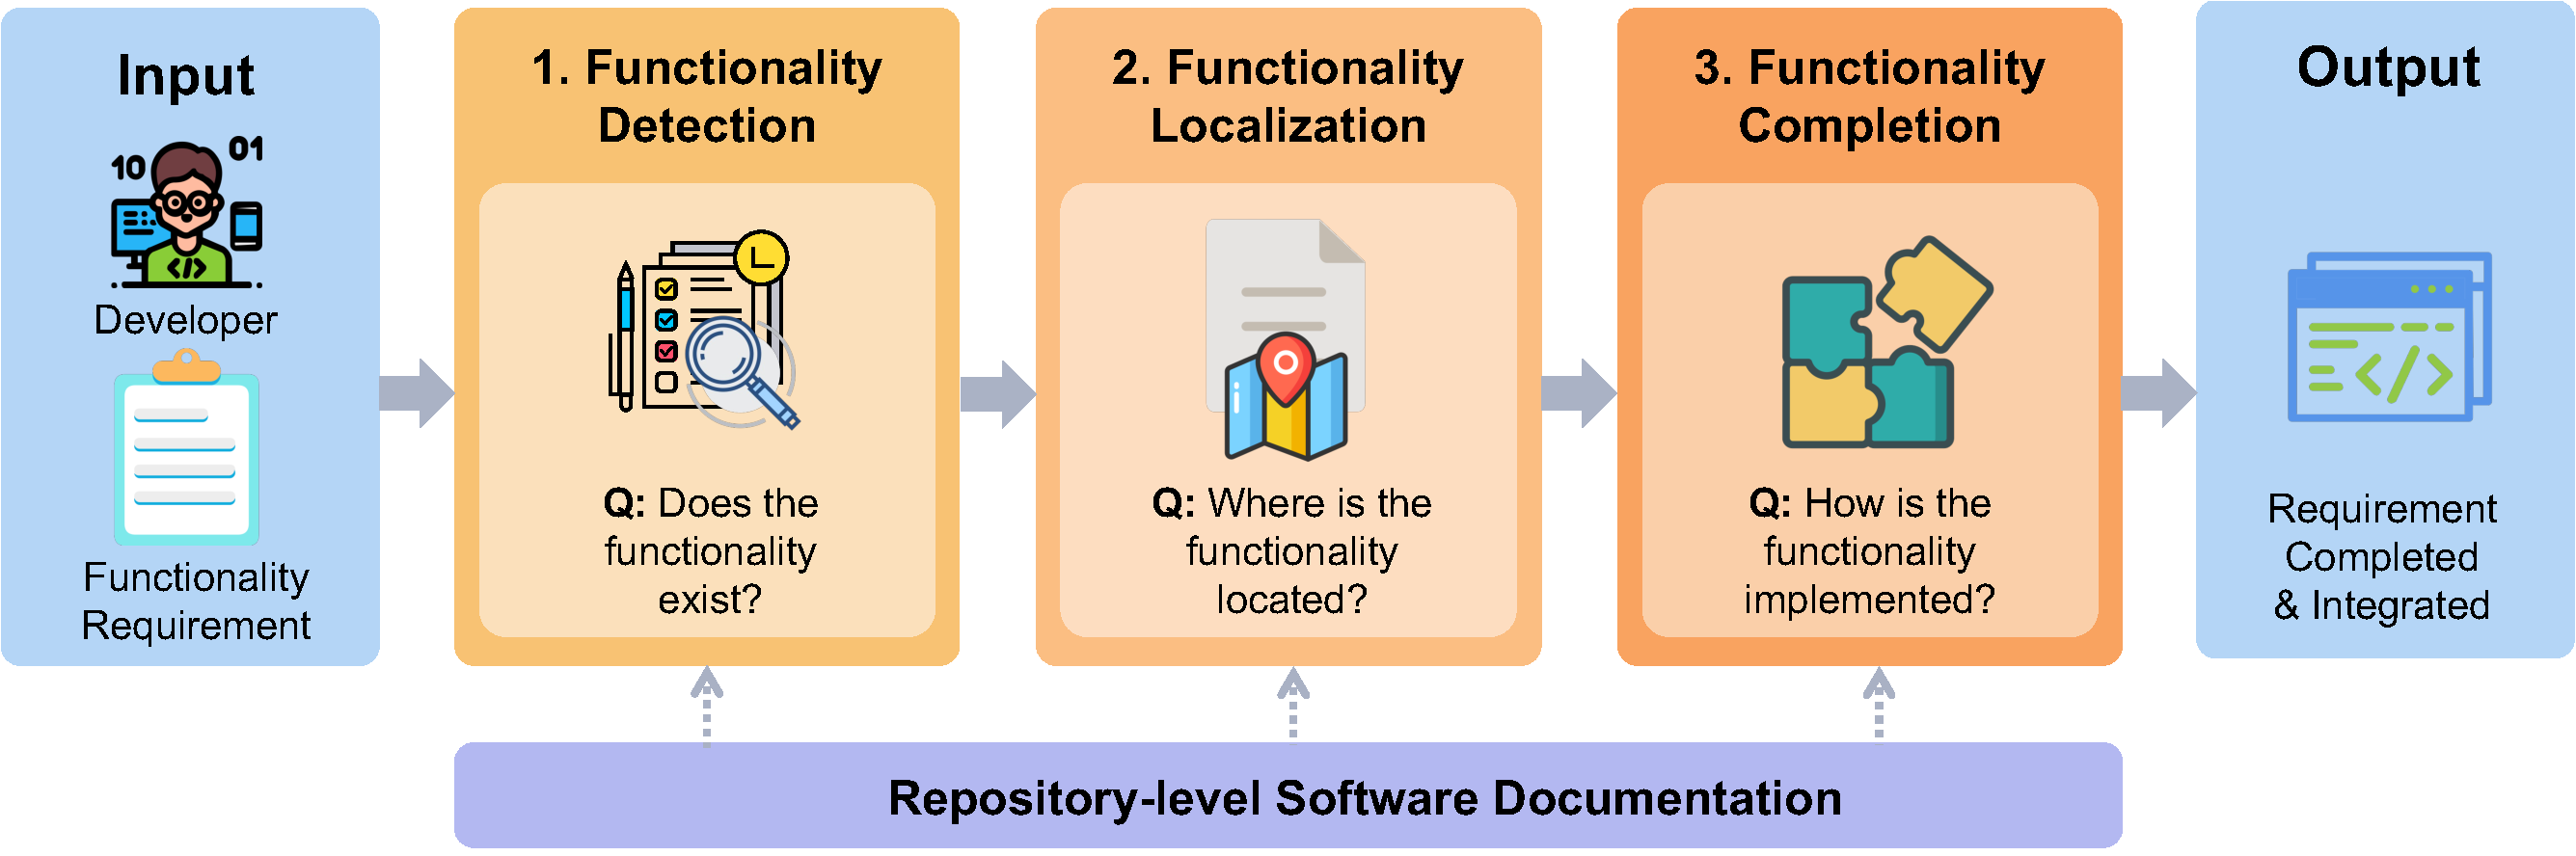
\includegraphics[width=.8\textwidth]{Figures/workflow.pdf}
    \vspace{-1.2em}
    \caption{A typical workflow of documentation-driven development.}
\label{fig:workflow}
\vspace{-1.5em}
\end{figure*}

Software documentation refers to describing the functionality and logic of source code, playing a crucial role in software engineering practices~\cite{survey1, survey4, survey5}. It facilitates developers' understanding of repositories, thereby enhancing development efficiency~\cite{survey2, survey3, heeager2012introducing, sommerville2001software, chomal2014significance}. Since manually writing documentation is costly, researchers have developed various automated methods. Early methods~\cite{template1, template2, info-retrieve1, info-retrieve2} are limited to summarizing isolated code snippets, such as functions or classes. They often neglect contextual information, including program dependency and functional interaction, resulting in fragmented documentation that provides limited guidance. With the advancement of large language models (LLMs), research has shifted towards generating repository-level documentation~\cite{docagent, repoagent}. These methods enhance documentation quality by retrieving semantic context from the entire repository to generate comprehensive summaries. AI-based assistants such as DeepWiki~\cite{deepwiki} and Autodoc~\cite{autodoc}, pre-generate software documentation for the user repository, thereby empowering diverse code tasks, such as code generation and issue solving.

Despite the progress in repository-level software documentation generation, existing benchmarks~\cite{repoagent, docagent, hierarchical} suffer from two fundamental limitations that hinder comprehensive evaluation: \textbf{(1) Lack of repository-level analysis:} Current benchmarks typically decompose generated documentation into function- or method-level summaries and assess them sequentially, overlooking semantic relationships between code snippets. This narrow focus does not well reflect real-world documentation reading, where developers rely on a holistic understanding to capture functionality spanning multiple modules. Hence, these benchmarks fail to assess the overall documentation accuracy. \textbf{(2) Unreliable evaluation strategy:} Current evaluation strategies generally fall into three types. Human-based methods~\cite{human1, human2} are labor-intensive, while metric-based methods~\cite{bleu,meteor,rouge} rely on reference documentation, which is generally difficult to construct. Hence, LLM-as-a-judge methods~\cite{docagent, hierarchical} are widely adopted due to their strong contextual understanding abilities. These methods typically utilize an LLM to assess documentation quality through a 5-point Likert scale~\cite{likert}. However, these scales rely on vague descriptors like ``not helpful'' and ``slightly helpful'', rather than a precise and objective definition. Besides, the LLM often lacks domain knowledge of the repository's implementation details, making it difficult to determine whether a documented functionality is accurately described. Furthermore, these strategies tend to assess the qualities of the documentation content, rather than its practical utility.

To mitigate these limitations, we propose a novel benchmark for evaluating repository-level \textbf{S}oft\textbf{W}are \textbf{D}ocumentation, named \textbf{\benchmark}. Our evaluation strategy is inspired by documentation-driven development~\cite{1377190, heeager2012introducing, survey2}, where higher-quality documentation enables developers to more effectively understand the repository. Figure~\ref{fig:workflow} illustrates a typical development workflow: when encountering functionality requirements, developers begin by searching the documentation to analyze whether the functionality has been implemented. If so, they then map the documentation descriptions to specific locations within the vast repository. Finally, developers leverage concrete information—such as API definitions and parameter usage—provided in the documentation to integrate the new functionality. Clearly, software documentation lies at the core of these consecutive stages. Based on this workflow, we simulate the LLM as a repository developer that understands and implements functionalities through a documentation-based inquiry process, instead of directly scoring the documentation. Accordingly, we construct three categories of repository-level, objective question-answering (QA) tasks aligned with this development workflow: \textbf{Functionality Detection}, \textbf{Functionality Localization}, and \textbf{Functionality Completion}. The documentation quality is measured by assessing the LLM's performance on these tasks. 

The construction pipeline of \benchmark is divided into three stages. (1) \textbf{\moduleA:} Pull Requests (PRs) typically introduce functionalities and contain rich contextual information, making them ideal for QA construction. Hence, we employ a series of rigorous crawling and filtering rules to retain high-quality PRs that genuinely reflect developers' functional contributions from representative repositories. (2) \textbf{\moduleB:} We enrich each PR with extensive contextual information, covering its background, motivation, and impact scope, such as program dependencies and associated issues. This comprehensive context provides a solid foundation for constructing repository-level QA tasks, thereby mitigating the limitation of insufficient analysis from a holistic perspective. (3) \textbf{\moduleC:} We leverage diverse context from PRs to meticulously create three categories of QA tasks. Each question is paired with a clear reference answer extracted from the PR's context. Based on this, we mitigate the limitation of unreliable evaluation strategies by assessing software documentation quality through the consistency between the LLM’s answers and the objective reference answers. \benchmark consists of 4,170 high-quality entries across three tasks. To ensure data quality, we manually validate a random sample of 100 entries, achieving a Kappa coefficient greater than 90\%, which indicates strong inter-annotator agreement. 
 
We conduct extensive experiments and conclude several findings:
\begin{enumerate}[leftmargin=*]
    \item There still exist limitations in current repository-level software documentation generation methods, among which methods leveraging more thorough context achieve better performance.
    \item Software documentation produced by the best method improves SWE-Agent's issue-solving rate by 20.00\%, highlighting its practical value in supporting documentation-driven development.
    \item Source code offers complementary value to software documentation on repository comprehension, especially in functionality detection and localization. 
\end{enumerate}

Our contributions can be summarized as follows:
\begin{enumerate}[leftmargin=*]
    \item We introduce \benchmark, a novel benchmark for evaluating repository-level software documentation. This benchmark aims to mitigate two major limitations, including the lack of repository-level analysis and unreliable evaluation strategies.
    \item \benchmark comprises 4,170 high-quality data entries. Each entry is enriched with three categories of functionality-driven QA tasks, enabling holistic and comprehensive evaluation of software documentation quality.
    \item We conduct extensive experiments on \benchmark, conclude our findings, and provide valuable insights for both researchers and developers.
\end{enumerate}